\newpage
\section{Globaler AIaaS-Markt}
Der globale Markt für Artificial Intelligence as a Service steigt immer weiter an. Die gesamte Marktgröße lag 2021 noch etwa bei 4,7 Milliarden US-Dollar, allerdings wird prognostiziert, dass der globale Markt bis 2030 auf ca. 92 Milliarden US-Dollar anwachsen könnte. Das entspräche, über einen Zeitraum von acht Jahren, einer durchschnittlichen jährlichen Wachstumsrate von 39,16 Prozent. Zu den wichtigsten Faktoren, die den Markt vorantreiben, gehören unter anderem der Bedarf und die Nachfrage an kostengünstigen KI-Lösungen von kleinen und mittelständigen Unternehmen, die Notwendigkeit die Markteinführungszeit von KI-Anwendungen zu verkürzen und der Mangel an Firmeninterner KI-Expertise. Zu den wichtigsten Akteuren auf dem Markt zählen Google LLC, IBM Corporation, Microsoft Corporation und Amazon Web Services Inc. All diese Akteure haben verschieden Konzepte, Herangehensweisen und Wachstumsstrategien wie Partnerschaften, Kooperationen und neue Produkteinführungen, um ihre Präsenz auf dem globalen Markt für künstliche Intelligenz als Dienstleistung zu etablieren und zu erweitern. Eine aussagekräftige Marktanalyse zu den jeweiligen Marktanteilen ist nicht möglich, da die Unternehmen ihre Umsatzzahlen im Bereich von AIaaS nicht einzeln veröffentlichen. Man weiß lediglich den gesamten Umsatz den sie mit künstlicher Intelligenz generieren, wovon AiaaS wohl nur ein Bruchteil davon ausmacht. \cite[vgl.][]{PR.2021} \\

\begin{figure}
  \centering
  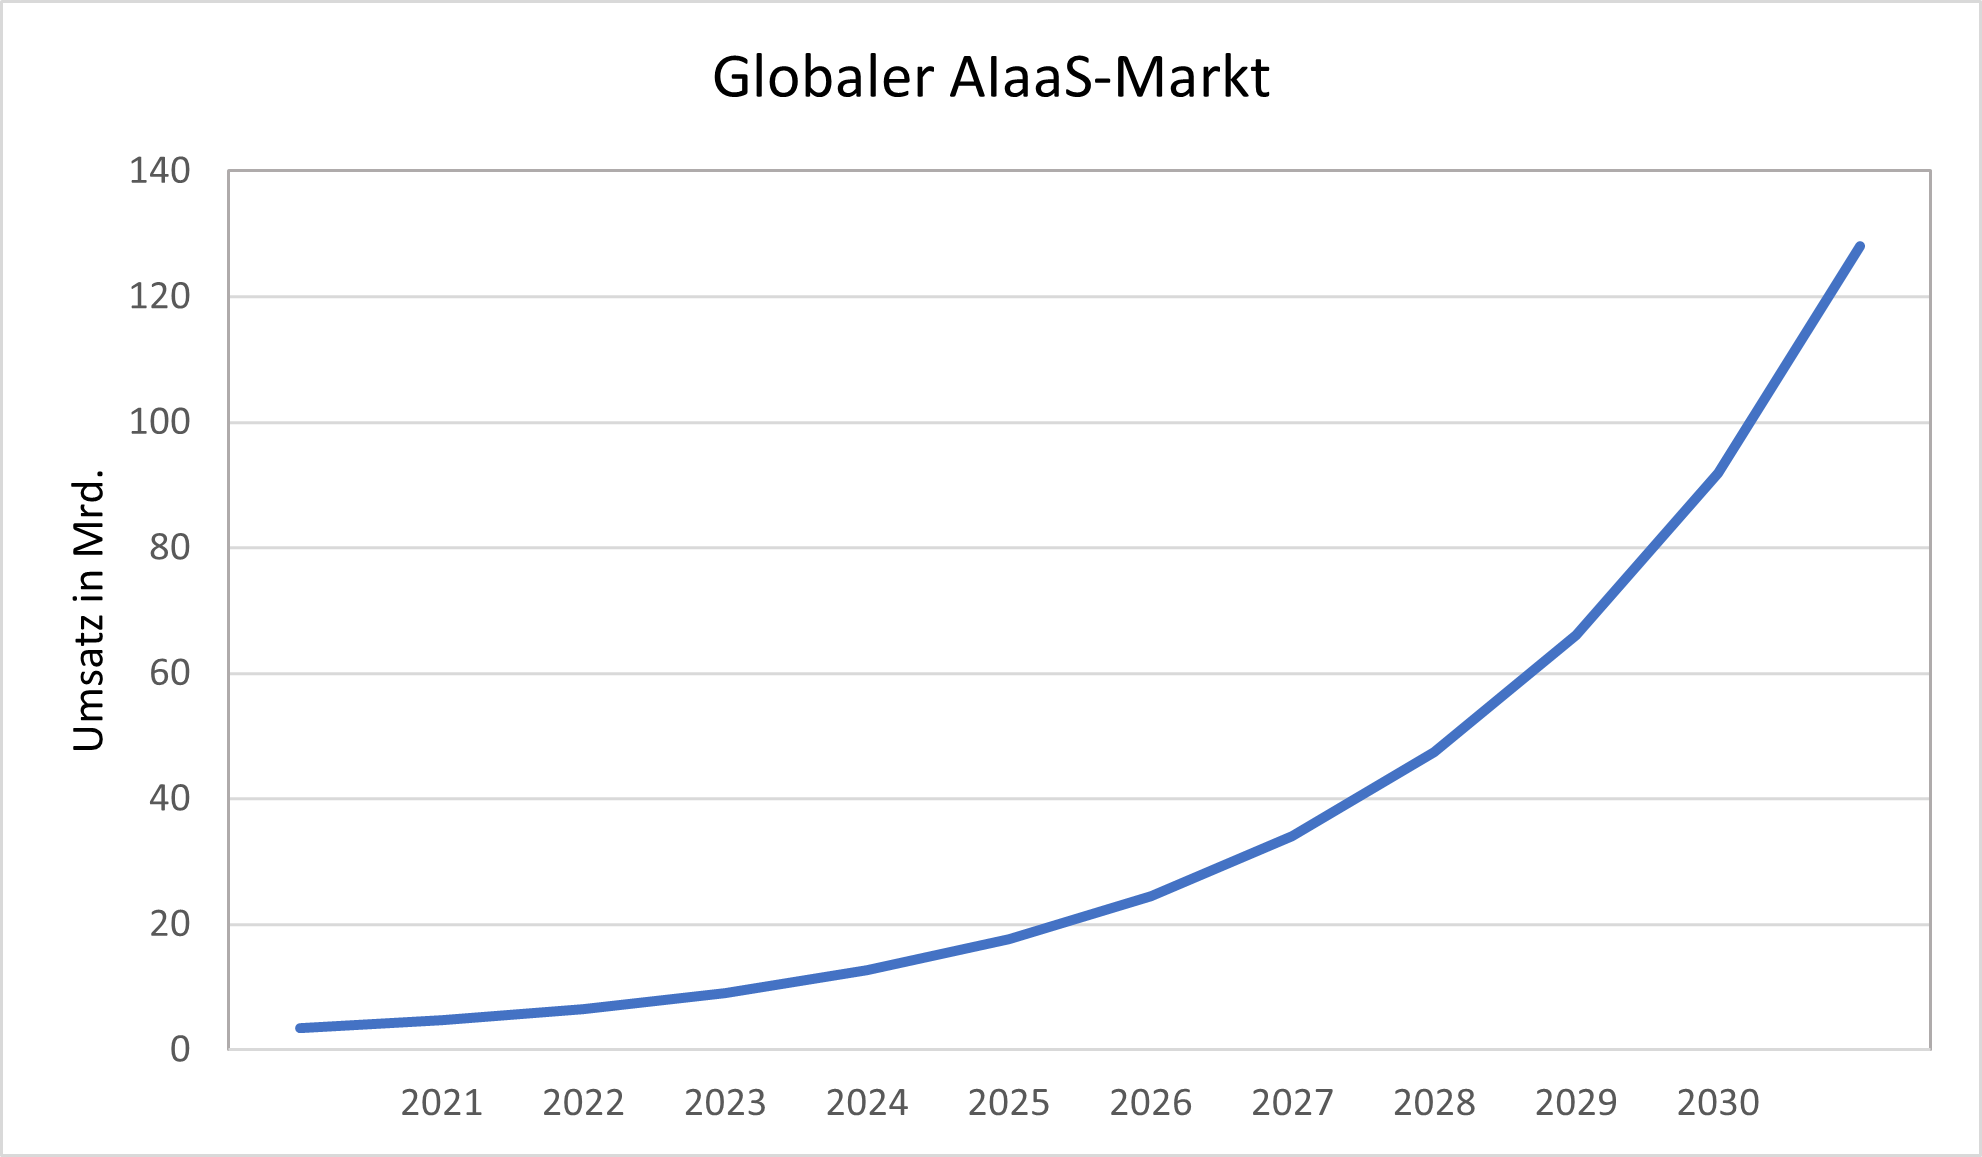
\includegraphics[width=\textwidth]{bilder/AIaaS-Markt.png}
  \caption{Prognostizierter, durchschnittlicher Marktverlauf bist 2030}
  \label{fig:aiaasmarkt}
\end{figure}


\subsection{Google LLC}
Google bietet eine Reihe von Diensten für künstliche Intelligenz an, mit denen Entwickler ihren Anwendungen problemlos intelligente Funktionen hinzufügen können. Zu diesen Diensten gehören vorab trainierte Modelle für maschinelles Lernen, die für Aufgaben wie Bilderkennung, Verarbeitung natürlicher Sprache und prädiktive Analysen verwendet werden können. Google bietet auch eine Cloudbasierte Entwicklungsumgebung für die Erstellung und das Training benutzerdefinierter maschineller Lernmodelle. Dieser Ansatz erleichtert Entwicklern den Einstieg in die KI, ohne dass sie in teure Hardware oder Software investieren müssen.
Zu den von Google angebotenen Produkten gehören unter anderem die Google Cloud Natural Language API, Cloud Speech API, Cloud Translation API und Cloud Vision API. Diese Dienste ermöglichen es Entwicklern, Anwendungen zu erstellen, die menschliche Sprache verstehen, Sprache in Text umwandeln, zwischen Sprachen übersetzen und Objekte in Bildern identifizieren können. Dabei können die Services mit einer simplen API-Anbindung in die eigenen Softwareprodukte eingebunden werden. \cite[vgl.][]{GoogleCloud.OA.2022}


\subsection{Microsoft Corporation}
Microsofts Ansatz für AIaaS bietet Entwicklern eine Reihe von Möglichkeiten, KI-Funktionen in ihre Anwendungen mit einzubinden. Dabei werden über eine cloudbasierte Plattform Bereiche wie die Bildverarbeitung, Sprachverarbeitung, Übersetzungen und Suchen bereitgestellt. Microsofts Ansatz für KI als Service zielt darauf ab, das Hinzufügen von KI-Fähigkeiten zu Anwendungen zu erleichtern, ohne dass dafür tiefgreifende KI-Kenntnisse erforderlich sind.  Das Unternehmen bietet auch eine Reihe von Tools und Ressourcen, die Entwickler für die Erstellung von KI-Anwendungen nutzen können, darunter zählt beispielsweise die Azure Machine Learning-Plattform.
Ein Key-Product von Microsoft im Bereich von Künstlicher Intelligenz als Service ist die Microsoft Azure Cognitive Services Suite. Diese stellt eine Reihe von APIs in den bereits genannten Gebieten: Bild- und Sprachverarbeitung, Übersetzungen und Suchen bereit, mit denen intelligente Funktionen durch einfache API-Anfragen in Anwendungen hinzugefügt werden können. Ein weiteres Produkt ist die Cortana Intelligence Suite. Diese umfasst intelligente Dienste zur Datenanalyse, zum maschinellen Lernen und zur Verarbeitung natürlicher Sprache. \cite[vgl.][]{Azure.OA.2022}

\newpage
\subsection{Amazon Web Services Inc.}
Amazons Ansatz der künstlichen Intelligenz als Service ist ein Cloud-basierter Dienst, der Entwicklern Tools zur Erstellung und Bereitstellung von KI-Anwendungen zur Verfügung stellt. Der Service bietet eine Vielzahl von Funktionen, darunter vortrainierte Modelle, eine benutzerfreundliche Oberfläche und Unterstützung für zahlreiche Programmiersprachen. Amazon bietet eine Reihe von KI-Diensten an, die es Entwicklern ermöglichen, anspruchsvolle Anwendungen mit Funktionen der künstlichen Intelligenz zu erstellen. Zu diesen Services gehören Amazon Lex, Amazon Polly, Amazon Rekognition und Amazon SageMaker. Amazon Lex ist ein Service, der es Entwicklern ermöglicht, Conversational Bots zu erstellen. Er nutzt die Verarbeitung natürlicher Sprache (NLP), um die Absichten der Benutzer zu verstehen und Benutzeranfragen zu erfüllen. Amazon Polly ist ein Text-to-Speech-Service, der Text in lebensechte Sprache umwandelt. Er unterstützt eine Reihe von Sprachen und kann verwendet werden, um Anwendungen zu erstellen, die sprechen. Das kann beispielsweise beim Erstellen einer Barrierefreien Software helfen. Amazon Recognition ist ein Bilderkennungsdienst, der zur Identifizierung von Objekten, Personen und Szenen in Bildern verwendet werden kann. \cite[vgl.][]{AWS.OA.2022}


\subsection{IBM Corporation}
Der IBM-Ansatz für künstliche Intelligenz als Service basiert auf der Watson-Plattform des Unternehmens. Neben der „klassischen“ Möglichkeit eigene KI-Modelle zu trainieren und sie dann in einer Cloud-Umgebung einzusetzen, umfasst die Plattform auch eine Reihe von APIs, die es Entwicklern ermöglicht, von ihren eigenen Anwendungen aus auf die Fähigkeiten von Watson zuzugreifen.
Einer der populärsten Bereiche, die die IBM Watson Services abdecken ist das maschinelle Lernen. Dabei wird Unternehmen die Möglichkeit geboten, automatisch aus Daten zu lernen und die eigenen Prozesse zu verbessern. Die Services nutzen eine Vielzahl von Algorithmen, um Unternehmen in die Lage zu versetzen, Vorhersagemodelle zu erstellen, die für eine Reihe von Aufgaben wie Betrugserkennung, Kundensegmentierung und vorausschauende Wartung verwendet werden können.
Ein weiteres wichtiges Segment ist die Verarbeitung natürlicher Sprache. Hier wird es zum einen ermöglicht, aus unstrukturierten Daten wie Text und Audio eine Bedeutung zu extrahieren. Es ist zum anderen aber auch möglich die Services für Stimmungsanalysen, Inhaltsklassifizierungen und Entitätsextraktion zu verwenden.
IBMs Lösungen für die Informationsextraktion aus Bildern nennt man IBM Computer Vision Services. Sie können für Aufgaben wie Objekterkennung, Bildklassifizierung und Bildsuche genutzt werden. \cite[vgl.][]{IBM.OA.2021} \\